\section{Построение и визуализация графа гиперссылок}
\paragraph{}
Процесс построения графа является одним из этапов конвеера обработки и происходит в \href{https://github.com/vasalf/hse-web-search-homework/blob/master/1/pipeline/graph_builder.py}{этом скрипте}. Скрипт создаёт в папке \textbf{result} файлы \textbf{graph\_full.gml} и \textbf{graph\_top.gml}. В файлах в формате GML (Graph Modelling Language) содержатся описания целого графа гиперссылок и подграфа из 150 наиболее популярных страниц.
\paragraph{Построение графа}

Этап построения графа является этапом конвеера обработки данных.

 При инициализации, создаётся пустой ориентированный граф, ассоциативные массивы из URL в целочисленные индексы и обратно, а так же пустое множество обработанных URL обработанных страниц. Для работы с графами использована библиотека \textbf{networkx}, выбранная из-за удобства создания и изменения графа и наличия графовых алгоритмов, в т.ч. PageRank.
 
 На этапе обработки веб-страницы на конвеере мы принимаем выделенную на предыдущем этапе метаинформацию о странице $i$, в которой содержится URL страницы и список URL всех гиперссылок со страницы. URL страницы нормализуется с помощью библиотеки \textbf{urllib}, добавляется в множество обработанных страниц, и ему присваивается уникальный индекс $p_i$. 
 
 Затем каждая гиперссылка $j$ со страницы нормализуется с помощью \textbf{urljoin} относительно базового URL страницы, и из полученного URL убираются все URL-фрагменты. К примеру, на странице \texttt{http://tut.by} гиперссылка \texttt{/index.php\#top} преобразуется в  \texttt{http://tut.by/index.php}. Затем ей присваивается уникальный индекс $p_j$ и в граф добавляется ребро $p_i \rightarrow p_j$.
 
 На этапе сохранения результата считается, что весь граф собран. Из него выделяется подграф на вершинах, являющихся обработанными страницами, таким образом, все внешние ссылки удаляются. Затем из него удаляются все вершины со степенью 0.
 
  Получившийся граф сериализуется в формат GML и сохраняется в \textbf{result/graph\_full.gml}. После этого на нём запускается алгоритм PageRank, и  в \textbf{result/graph\_top.gml} сохраняется подграф на 150 вершинах с максимальным рейтингом PageRank.
 \paragraph{Результаты}
 В итоговом графе содержится 165149 вершин и 1007123 рёбер. Компонент слабой связности всего 4192. В подграфе из 150 вершин с максимальным PageRank 150 вершин и 328 рёбер, 22 компоненты слабой связности. 
 \paragraph{Визуализация}
 Для визуализации использовался инструмент \textbf{Gephi}. Для укладки использовался алгоритм Fruchtermann-Reingold. Вершины и ребра раскрашены в соответствии с компонентой слабой связности, размер вершины пропорционален её PageRank. Граф всех вершин можно увидеть на рисунке \ref{graph-all}, топ-150 Pagerank - на рисунке \ref{graph-top} 
 
 \begin{figure}[h]
 	
\includegraphics[width=.5\textwidth]{graph_all.jpeg}
 	\caption{Граф гиперссылок}
 	\label{graph-all}
 \end{figure}
 
 \begin{figure}[h]
 	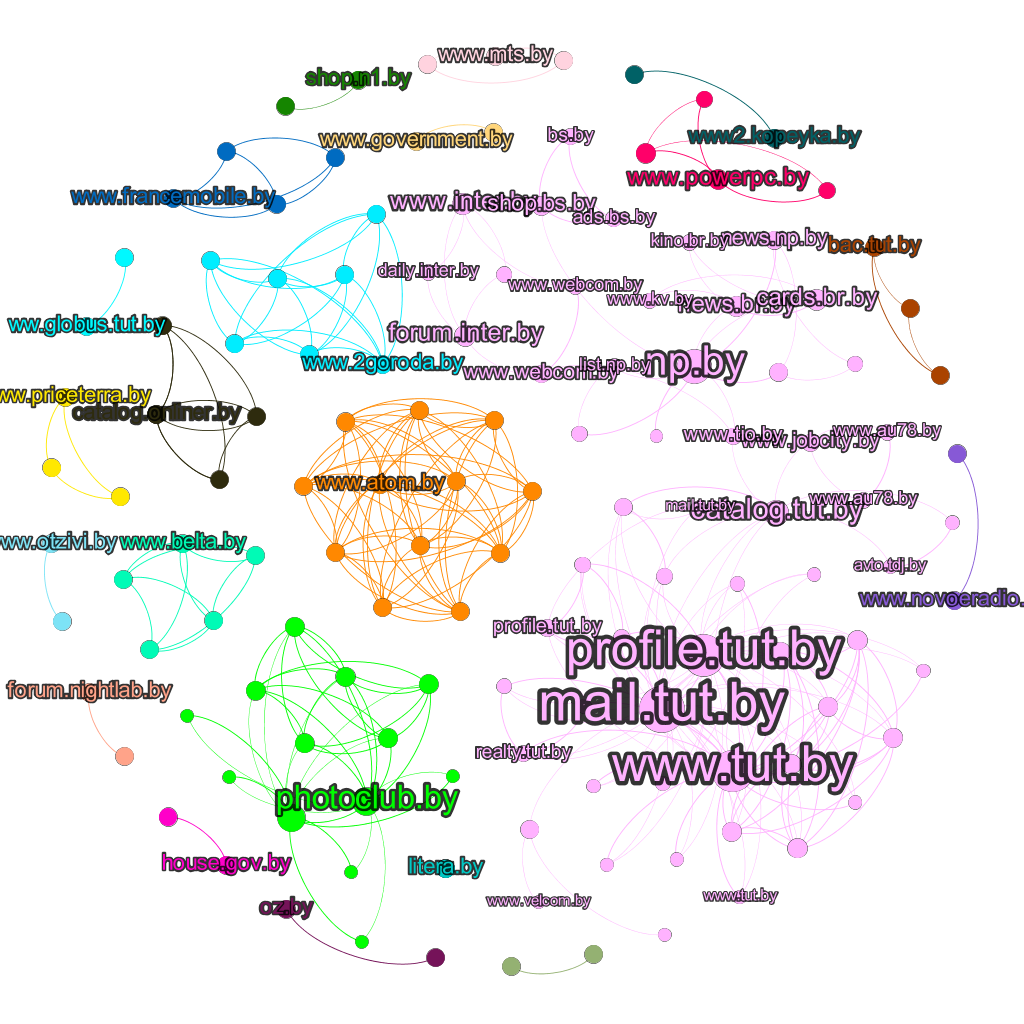
\includegraphics[width=.5\textwidth]{graph_top_white.png}
 	\caption{Граф гиперссылок, топ-150 PageRank}
 	\label{graph-top}
 \end{figure}
 